\section{Training Results}

\begin{figure}[!htbp]
\centering
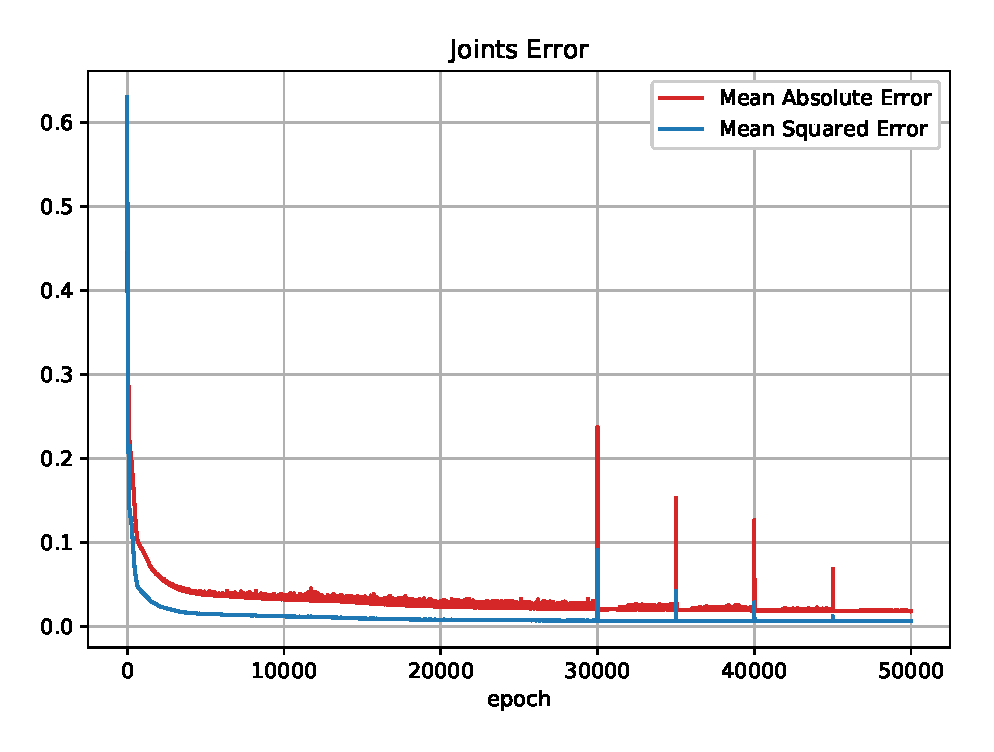
\includegraphics[width=1\textwidth]{Cap6/errors}
\caption{Plots of mean squared error and mean absolute error, during training.}
\label{fig:errors}
\end{figure}

The initial results came from the training procedure, outside the simulation environment. Figure \ref{fig:errors} presents training curves for the kick keyframe dataset. In this case, plots show the mean squared error and the mean absolute error metrics. In both metrics, the value drastically decreases in the first epochs. This same behavior was present in other training procedures as well. However, only after thousands of epochs, the network has achieved a low error that successfully reproduced the motion, which has shown how sensible to small joint errors keyframes were, given that they were open-loop motions. The peaks, during the training has happened at the learning rate transition instants, but they did not hurt the training procedure itself.

\section{The Learned Kick Motion}

The final mean absolute error was \textbf{0.018} radians and the motion was visually indistinguishable from the original one, as can be seen in Figure \ref{fig:motions}. In this figure, snapshots from both motions were taken. Figure \ref{fig:kick_joints_curves} shows several plots of joint angles, by comparing the original and learned kick motions. As we may see, the learned motion has fitted the movement with minor errors\footnote{\label{footnote_walk} Kick results video: https://youtu.be/UAbqQLUnvDo}.

\begin{figure}[!htbp]
\centering
\includegraphics[angle=90,width=1\textwidth]{Cap6/motions}
\caption{The kick motion. The first row of figures shows the original kick motion. The second row shows the learned kick motion. Both motions are visually indistinguishable.}
\label{fig:motions}
\end{figure} 

In order to evaluate the learned kick motion in the RoboCup Soccer 3D domain, we created a statistical test. Inside the test scenario, the ball was initially placed in the center of the field with an agent near to it. The only action of the agent was to kick the ball in the goal direction. After the kick, the agent run until reaching the ball and kicked it again, repeating this process till scoring a goal. When the goal has occurred, this same scenario was repeated. The whole test was conducted, during thirty minutes in clock time and the following data was collected: total number of kicks, number of successful kicks, mean distance that the ball has traveled, and the standard deviation of this measure. The results from the original and learned kicks is shown in Table \ref{tab_kicks_statistics}.


\begin{figure*}[!htbp]
\centering
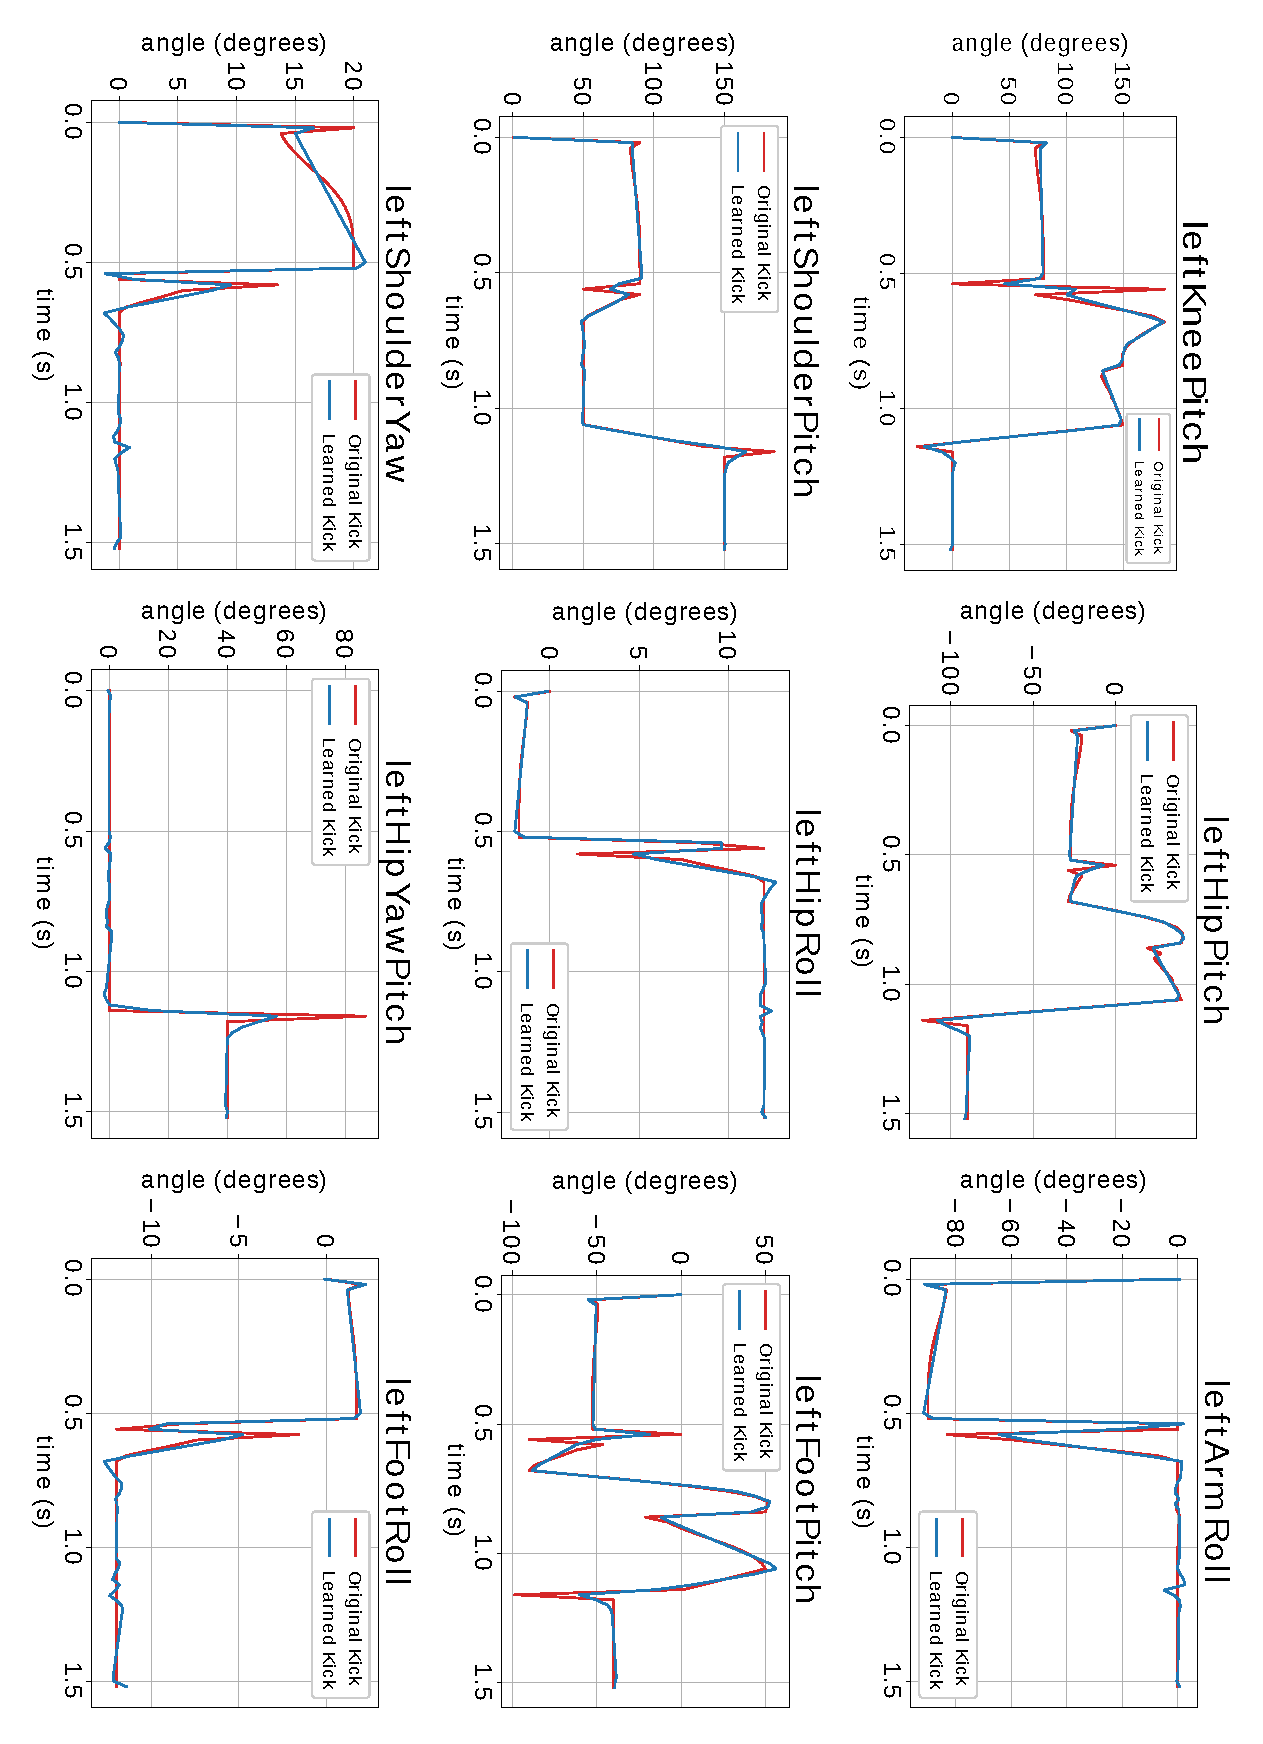
\includegraphics[angle=90,width=1\textwidth]{Cap6/kick_joints_curve}
\caption{Joint values for comparing original and learned kicks. The neural network was able to fit the joint trajectories with small errors.}
\label{fig:kick_joints_curves}
\end{figure*}


\begin{table}[htbp]
\caption{The Kick Comparison}
\begin{center} 
\begin{tabular}{|c|c|c|c|}
\hline
\textbf{Kick}&\multicolumn{3}{|c|}{\textbf{Statistics}} \\
\cline{2-4} 
\textbf{Type} & \textbf{\textit{Accuracy (\%)}}& \multicolumn{2}{|c|}{\textbf{Distance (\(m\))}} \\ 
\cline {3-4}
& & \textbf{\textit{Mean}}& \textbf{\textit{Std}} \\
\hline
Original Kick & 64.5 & 8.92 & 3.82  \\
\hline
Neural Kick & 52.6 & 7.16 & 4.06 \\
\hline
\end{tabular}
\label{tab_kicks_statistics}
\end{center}
\end{table}

Although both kicks had similar results, the original kick was slightly better in this scenario. By confronting Figure \ref{fig:kick_joints_curves}, we can conclude that even with an almost equal representation, the kick lost part of its efficiency and this fact has shown how sensible were movements based on keyframe data.

\section{The Learned Walk Motion}
By using the modified server described in Subsec. \ref{AA}, a dataset with samples of the UT Austin Villa's walking motion \cite{macalpine2013} was acquired. This team is the current champion of the RoboCup Soccer 3D competition \cite{macalpine2017}.

The objective was to mimic the walk motion as a keyframe and has used that in our agent. The previously described framework for learning our own kick motion was used in this training, by including the neural network architecture and its hyperparameters.

The results from this training are shown in Figure \ref{fig:walk_joints_curves}. Similarly to Figure \ref{fig:kick_joints_curves}, it shows the joint angles throughout the walking motion period for the original and learned walk. Additionally, it shows the real joints values from the movement in the server. These joints were chosen because they were the most dynamic in the walk motion and, therefore, the hardest to learn.

\begin{figure*}[!htbp]
\centering
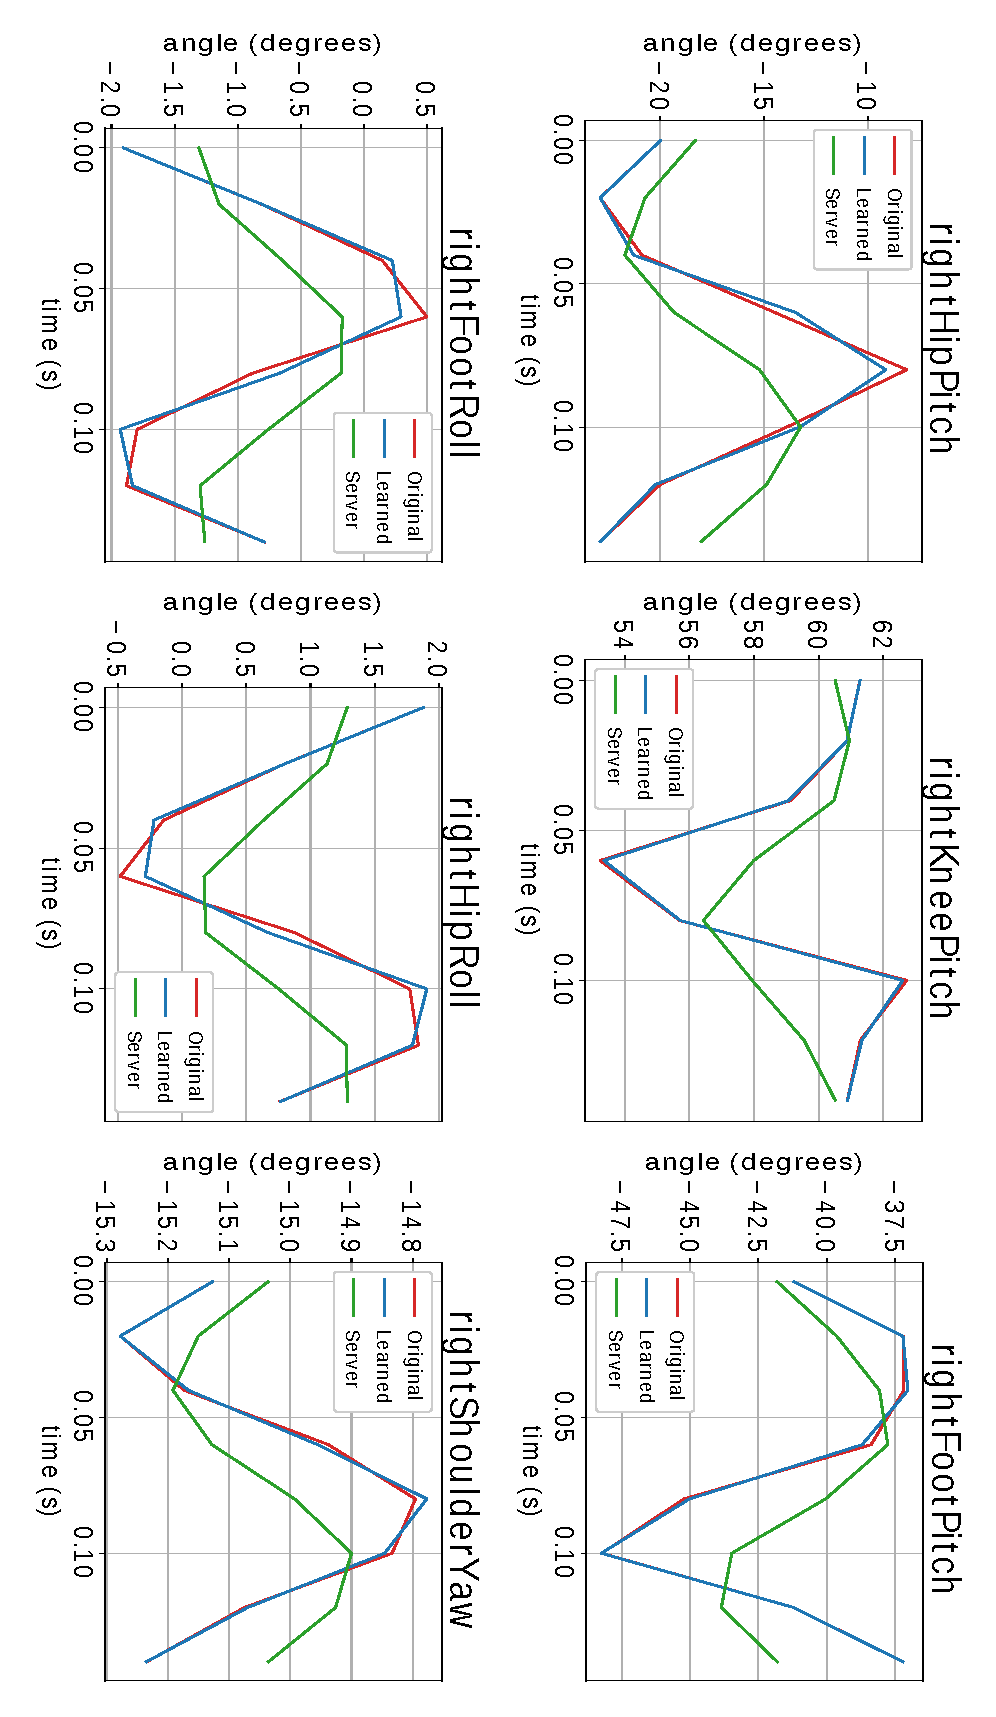
\includegraphics[angle=90,width=1\textwidth]{Cap6/walk_joints_curves}
\caption{Joints positions, during a period of the walking motion for the original walk, and the learned walk and the joints positions effectively attained, during the learned walking motion.}
\label{fig:walk_joints_curves}
\end{figure*}

The learned motion has fitted the dataset very well. However, these values were just desired joints. In fact, these values were used as references to joint controllers and were also attenuated due to joint dynamics. Furthermore, this motion was operated in a open-loop fashion, so the agent was not able to correct its own trajectory, and this walks got biased within the simple task of walking straight forward.

Despite the facts previously described, the motion has worked well in a non-competitive scenario\footnote{\label{footnote_walk} Walk results video: https://youtu.be/-pHxTrxllyY}, which was shown in the metrics collected from the Forward Walk test scenario -- agent walking forward from the goal post until the center line of the field -- in Table \ref{tab_walk} and the visual representation in Figure \ref{fig:walkings}.

\begin{table}[htbp]
\caption{Walk Comparison - Forward Walk}
\begin{center}
\begin{tabular}{|c|c|c|c|c|}
\hline
\textbf{Walk}&\multicolumn{4}{|c|}{\textbf{Statistics}} \\
\cline{2-5} 
\textbf{Type} &\multicolumn{2}{|c|}
{\textbf{Velocity \((m/s)\)}}
&\multicolumn{2}{|c|}{\textbf{Y Error \( (m) \) }} \\ 
\hline
 &
\textbf{\textit{Mean}} &
\textbf{\textit{Std}} & \textbf{\textit{Mean}} & \textbf{\textit{Std}} \\
\hline
Original Walk & 0.87 & 0.01 & - & -  \\
\hline
Learned Walk & 0.23 & 0.01 & 0.96 & 2.63 \\
\hline
\end{tabular}
\label{tab_walk}
\end{center}
\end{table}


\begin{figure}[!htbp]
\centering
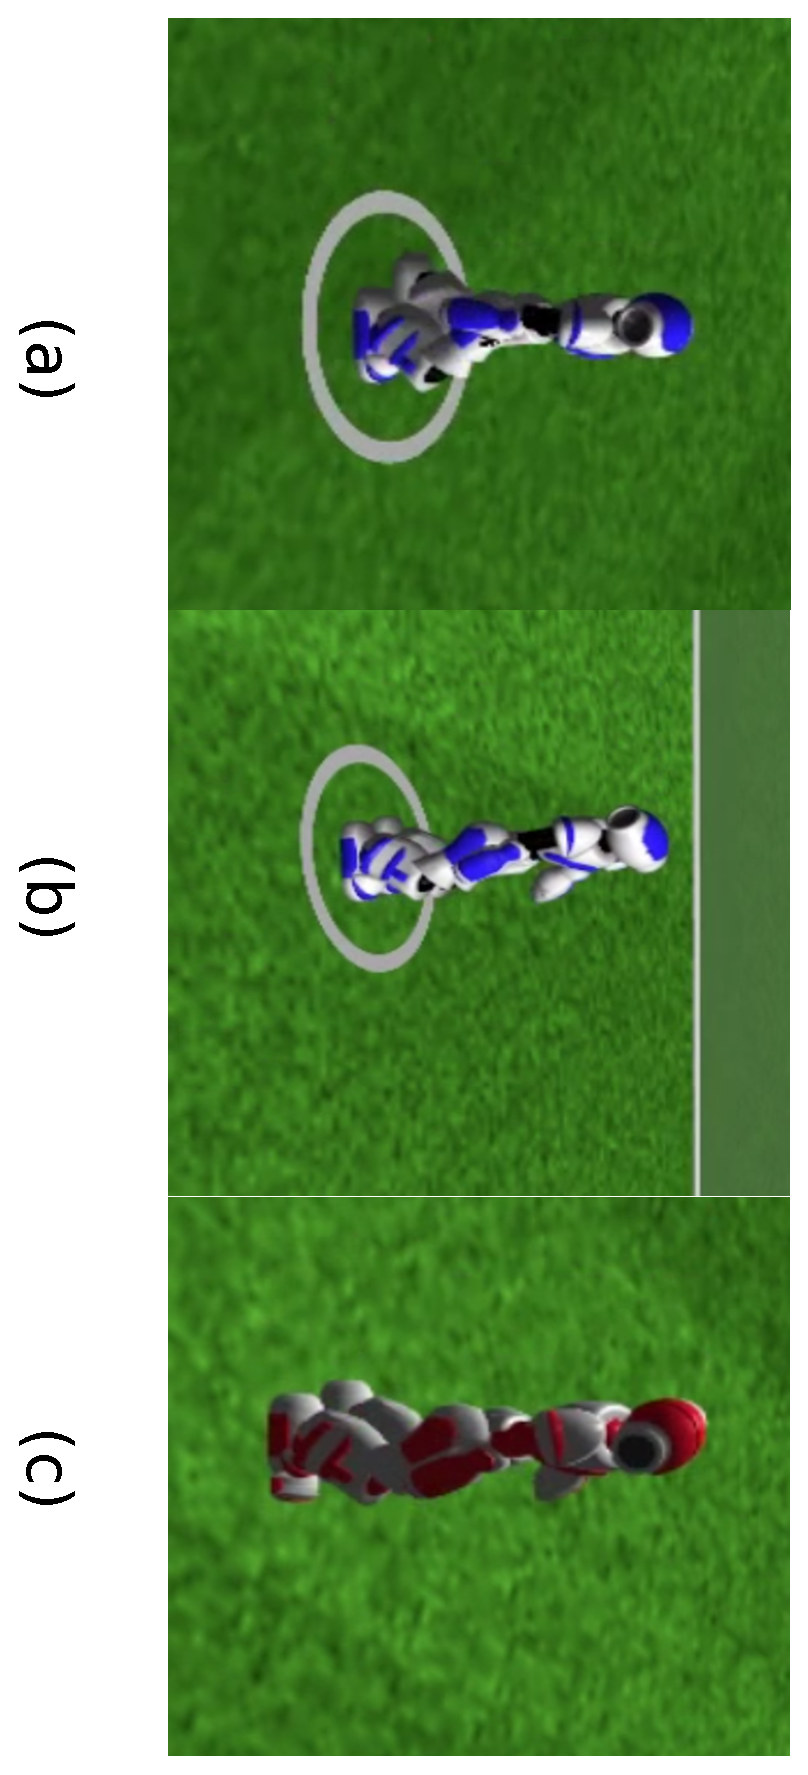
\includegraphics[angle=90, width=1\textwidth]{Cap6/walkings}
\caption{The walking motions comparison. Figure (a) shows our agent in its regular walk, Figure (b) shows the same agent mimicking UT Austin Villa walk, and Figure (c) shows the UT Austin Villa agent itself performing his own walking motion.}
\label{fig:walkings}
\end{figure}

\section{Other motions}

This same framework was used to learn other keyframe motions originated from our agent itself, such as the get up motion. As the cases previously described, the resultant neural network was capable of mimicking the keyframe, by including its interpolation. Hence, all of our keyframe motions could be replaced by neural motions with similar performance.

However, the huge improvement of this method was about mimicking other teams motions. In the Soccer 3D environment, movements like kick and walking have giant impact in team's performance. With this learning framework, our agent was able to mimic multiples movements from several teams.

As an example, we have collected data from UT Austin Villa kick, which was originally optimized by using Deep Reinforcement Learning techniques \cite{mcalpine2017}. Our agent has learned this kick without any additional optimization strategy: we just have used samples collected from the modified server.

